\documentclass[compress,mathserif,cjk]{beamer}
\usepackage{mathrsfs}
\usepackage{color}
\usepackage{CJK}
\usepackage{amssymb}
\usepackage{amsmath}
\usepackage{extarrows}
\usepackage{ulem}
\usepackage{latexsym}
\usepackage{pmat}

% Copyright 2003 by Till Tantau <tantau@cs.tu-berlin.de>.
%
% This program can be redistributed and/or modified under the terms
% of the LaTeX Project Public License Distributed from CTAN
% archives in directory macros/latex/base/lppl.txt.

%
% The purpose of this example is to show how \part can be used to
% organize a lecture.
%
\usetheme{Warsaw}
  % 可供选择的主题参见 beameruserguide.pdf, 第 134 页起
  % 无导航条的主题: Bergen, Boadilla, Madrid, Pittsburgh, Rochester;
  % 有树形导航条的主题: Antibes, JuanLesPins, Montpellier;
  % 有目录竖条的主题: Berkeley, PaloAlto, Goettingen, Marburg, Hannover;
  % 有圆点导航条的主题: Berlin, Dresden, Darmstadt, Frankfurt, Singapore, Szeged;
  % 有节与小节导航条的主题: Copenhagen, Luebeck, Malmos, Warsaw

%  \setbeamercovered{transparent}
% 如果取消上一行的注解 %, 就会使得被覆盖部分变得透明(依稀可见)

\usepackage[english]{babel}
\usepackage[latin1]{inputenc}
\usepackage{CJK}

%\usepackage{beamerthemesplit}
%\usepackage{beamerthemeshadow,color}
\usepackage{pgf,pgfarrows,pgfnodes,pgfautomata,pgfheaps,pgfshade}
\usepackage{amsmath,amssymb}
\usepackage{bm}
\usepackage{colortbl}

\graphicspath{{images/}}         %% 图片路径. 本文的图片都放在这个文件夹里了.
\DeclareGraphicsRule{*}{mps}{*}{} %% 使 pdflatex 可以纳入 metapost 做的图片.
\renewcommand{\div}{\operatorname{div}}
\renewcommand{\raggedright}{\leftskip=0pt \rightskip=0pt plus 0cm}
\raggedright %% 中文对齐

%==============自定义: 逐个 item 高亮(\hilite), 或"高黑"(\hidark)==================%
\def\hilite<#1>{%
\temporal<#1>{\color{blue!35}}{\color{magenta}}%
{\color{blue!75}}}
\def\hidark<#1>{%
\temporal<#1>{\color{black!35}}{\color{magenta}}%
{\color{black}}}

\newcolumntype{H}{>{\columncolor{blue!20}}c!{\vrule}}
\newcolumntype{H}{>{\columncolor{blue!20}}c}  %% 表格设置
%==================================参考文献==============================================================
\newcommand{\upcite}[1]{\textsuperscript{\cite{#1}}}  %自定义命令\upcite, 使参考文献引用以上标出现
\bibliographystyle{plain}
%=========================================================================================

\def\colorb{\textcolor[rgb]{0.00,0.00,1.00}}
\def\colorg{\textcolor[rgb]{0.00,1.00,0.00}}
\def\colorr{\textcolor[rgb]{1.00,0.00,0.00}}
\newcommand\hdim{\dim_{\mathrm H}}
\newtheorem{lem}{Lemma}[section]
\newtheorem{nt}[lem]{Notation}
\newtheorem{dfn}[lem]{Definition}
\newtheorem{pro}[lem]{Proposition}
\newtheorem{thm}[lem]{Theorem}
\newtheorem{exa}[lem]{Example}
\newtheorem{cor}[lem]{Corollary}
\theoremstyle{remark}
\newtheorem*{rem}{Remark}
\numberwithin{equation}{section}
\def\N{\mathbb N}
\def\Q{\mathbb Q}
\def\R{\mathbb R}
\def\Z{\mathbb Z}
\def\vep{\varepsilon}
%=========================================================================================
%\setbeamercovered{transparent}
%
% The following info should normally be given in you main file:
%

%%%%%%%%%%%%%%%%%%%%%%%%%%%%%%%%%%%%%%%%%%%%%%%%%%%%%%%%%%%%%%%%%%%%%%%%%%%%%%%%%%%%%%%%%%%%%%%%%%%%%%%%%
%                                           定制幻灯片---重定义字体、字号命令                           %
%%%%%%%%%%%%%%%%%%%%%%%%%%%%%%%%%%%%%%%%%%%%%%%%%%%%%%%%%%%%%%%%%%%%%%%%%%%%%%%%%%%%%%%%%%%%%%%%%%%%%%%%%
\newcommand{\song}{\CJKfamily{song}}    % 宋体   (Windows自带simsun.ttf)
\newcommand{\fs}{\CJKfamily{fs}}        % 仿宋体 (Windows自带simfs.ttf)
\newcommand{\kai}{\CJKfamily{kai}}      % 楷体   (Windows自带simkai.ttf)
\newcommand{\hei}{\bf}      % 黑体   (Windows自带simhei.ttf)
\newcommand{\li}{\CJKfamily{li}}        % 隶书   (Windows自带simli.ttf)
\newcommand{\you}{\CJKfamily{you}}      % 幼圆   (Windows自带simyou.ttf)
\newcommand{\chuhao}{\fontsize{42pt}{\baselineskip}\selectfont}     % 字号设置
\newcommand{\xiaochuhao}{\fontsize{36pt}{\baselineskip}\selectfont} % 字号设置
\newcommand{\yichu}{\fontsize{32pt}{\baselineskip}\selectfont}      % 字号设置
\newcommand{\yihao}{\fontsize{28pt}{\baselineskip}\selectfont}      % 字号设置
\newcommand{\erhao}{\fontsize{21pt}{\baselineskip}\selectfont}      % 字号设置
\newcommand{\xiaoerhao}{\fontsize{18pt}{\baselineskip}\selectfont}  % 字号设置
\newcommand{\sanhao}{\fontsize{15.75pt}{\baselineskip}\selectfont}  % 字号设置
\newcommand{\sihao}{\fontsize{14pt}{\baselineskip}\selectfont}      % 字号设置
\newcommand{\xiaosihao}{\fontsize{12pt}{\baselineskip}\selectfont}  % 字号设置
\newcommand{\wuhao}{\fontsize{10.5pt}{\baselineskip}\selectfont}    % 字号设置
\newcommand{\xiaowuhao}{\fontsize{9pt}{\baselineskip}\selectfont}   % 字号设置
\newcommand{\liuhao}{\fontsize{7.875pt}{\baselineskip}\selectfont}  % 字号设置
\newcommand{\qihao}{\fontsize{5.25pt}{\baselineskip}\selectfont}    % 字号设置

%======================= 标题名称中文化 ============================%
\newtheorem{dingyi}{\hei 定义~}[section]
\newtheorem{dingli}{\hei 定理~}[section]
\newtheorem{yinli}[dingli]{\hei 引理~}
\newtheorem{tuilun}[dingli]{\hei 推论~}
\newtheorem{mingti}[dingli]{\hei 命题~}
%%%%%%%%%%%%%%%%%%%%%%%%%%%%%%%%%%%%%%%%%%%%%%%%%%%%%%%%%%%%%%%%%%%%%%%%%%%%%%%%%%%%%%%

% \usepackage{beamerthemesplit} // Activate for custom appearance


\title{\textsc{第6章\ \ \ 二次型}}
\author{郑州大学数学与统计学院 线性代数教研室}
\date{}

\begin{document}
\begin{CJK}{UTF8}{gbsn}
\frame{\titlepage}

\begin{frame}\frametitle{目录}
 \tableofcontents
\end{frame}
%%%%%%%%%%%%%%%%%%%%%%%%%%%%%%%%%%%%%%%%%%%%%%%%%%%%%%%%%%%%%%%%%%%%%%%%%%%%%%%%%%%%%%

\section[6.1]{6.1 二次型及其矩阵表示}

\begin{frame}{二次型的概念}
 \ \ \ \ {\hei 定义~6.1} 设$P$是数域,则含有$n$个变量(或称文字)的二次齐次多项式
 \begin{eqnarray*}
 f(x_1,x_2,\cdots,x_n)&=&a_{11}x_1^2+2a_{12}x_1x_2+\cdots+2a_{1n}x_1x_n\\
 &&\hspace{4em}~+a_{22}x_2^2+\cdots+2a_{2n}x_2x_n\\
 &&\hspace{7em}~~~+\cdots\\
 &&\hspace{12em}+a_{nn}x_n^2
 \end{eqnarray*}
 其中$a_{ij}(i,j=1,2,\cdots,n)\in P$不全为0,称为数域$P$上的一个$n${\hei 元二次型},简称{\hei 二次型}。如果$f$为零多项式,也称$f$为数域$P$上的一个二次型,叫做{\hei 零二次型}。
 \pause\vskip 5pt
 \ \ \ \ 若$P$是实数域,则称$f$为{\hei 实二次型};若$P$是复数域,则称$f$为{\hei 复二次型}。只含平方项的二次型称为{\hei 标准二次型},简称{\hei 标准形}。
\vskip 50pt\
\end{frame}

\begin{frame}
\ \ \ \ {\hei 例~1} $f_1(x,y)=x^2+xy+2y^2,~f_2(x)=2x^2,~f_3(x_1,x_2,x_3)=\frac{x_1^2}{a^2}+\frac{x_2^2}{b^2}+\frac{x_3^2}{c^2}$都是二次型,其中$f_2$和$f_3$是标准形。

\end{frame}

\begin{frame}{二次型的矩阵表示}\small
 在二次型$f$的表达式中令$a_{ij}=a_{ji}$,则有
 \begin{eqnarray*}
 f(x_1,x_2,\cdots,x_n)&=&~~~a_{11}x_1^2+a_{12}x_1x_2+a_{13}x_1x_3+\cdots+a_{1n}x_1x_n\\
 &&+a_{21}x_2x_1+a_{22}x_2^2+a_{23}x_2x_3+\cdots+a_{2n}x_2x_n\\
 &&+\cdots\\
 &&+a_{n1}x_nx_1+a_{n2}x_nx_2+a_{n3}x_nx_3+\cdots+a_{nn}x_n^2
 \end{eqnarray*}
 即
 $$f(x_1,x_2,\cdots,x_n)=\sum_{i=1}^n\sum_{j=1}^na_{ij}x_ix_j.$$
 \pause 若令
 $$\bm A=\left[\begin{matrix}a_{11}&a_{12}&\cdots&a_{1n}\\a_{21}&a_{22}&\cdots&a_{2n}\\\vdots&\vdots&&\vdots\\a_{n1}&a_{n2}&\cdots&a_{nn}\end{matrix}\right],~~~
 \bm X=\left[\begin{matrix}x_1\\x_2\\\vdots\\x_n\end{matrix}\right],$$
 \end{frame}

\begin{frame}\small
则$\bm A$为对称矩阵,且二次型$f$可化为
\begin{eqnarray*}
 f(x_1,x_2,\cdots,x_n)&=&(x_1,x_2,\cdots,x_n)\left[\begin{matrix}a_{11}x_1+a_{12}x_2+\cdots+a_{1n}x_n\\a_{21}x_1+a_{22}x_2+\cdots+a_{2n}x_n\\\vdots\\
 a_{n1}x_1+a_{n2}x_2+\cdots+a_{nn}x_n\end{matrix}\right]\\
 &=&(x_1,x_2,\cdots,x_n)\left[\begin{matrix}a_{11}&a_{12}&\cdots&a_{1n}\\a_{21}&a_{22}&\cdots&a_{2n}\\\vdots&\vdots&&\vdots\\a_{n1}&a_{n2}&\cdots&a_{nn}\end{matrix}\right]
 \left[\begin{matrix}x_1\\x_2\\\vdots\\x_n\end{matrix}\right]\\
 &=&\bm X'\bm{AX},
\end{eqnarray*}
即
$$f(x_1,x_2,\cdots,x_n)=\bm X'\bm{AX}.$$
上式称为二次型$f$的{\hei 矩阵表达式},$\bm A$称为{\hei 二次型的矩阵}。
\end{frame}

\begin{frame}
 \ \ \ \ {\hei 说明} 对一般方阵$\bm A$
 $$f(x_1,x_2,\cdots,x_n)=\bm X'\bm{AX}=\sum_{i=1}^na_{ii}x_i^2+\sum_{1\leq i<j\leq n}(a_{ij}+a_{ji})x_ix_j$$
 也是一个二次型。\pause 这时有$f(x_1,x_2,\cdots,x_n)=\bm X'\Big(\frac{\bm A+\bm A'}2\Big)\bm X$.
 \pause\vskip 15pt
\ \ \ \ {\hei 例~2} 写出$f(x_1,x_2,x_3)=2x_1^2+x_1x_2+x_2x_3+x_3^2$的矩阵$\bm A$.
\pause\vskip 10pt
\ \ \ \ {\hei 例~3} 写出对称矩阵$\bm A=\left[\begin{matrix}1&2&1\\2&-2&3\\1&3&0\end{matrix}\right]$所对应的二次型$f(x,y,z)$.
\end{frame}

\begin{frame}{标准二次型的矩阵表示}
\ \ \ \ 标准二次型
$$f(x_1,x_2,\cdots,x_n)=\lambda_1x_1^2+\lambda_2x_2^2+\cdots+\lambda_nx_n^2$$
的矩阵表达式是
$$\bm X'\bm{AX}=[x_1,x_2,\cdots,x_n]\left[\begin{matrix}\lambda_1&&&\\&\lambda_2&&\\&&\ddots&\\&&&\lambda_n\end{matrix}\right]\left[\begin{matrix}x_1\\x_2\\\vdots\\x_n\end{matrix}\right].$$
可见标准形的矩阵是对角矩阵。反之,对角矩阵对应的二次型是标准形。
\pause\vskip 10pt
\ \ \ \ {\hei 定义~6.2} 二次型$f=\bm X'\bm{AX}$的矩阵$\bm A$的秩称为{\hei 二次型的秩}。
\end{frame}

\section[6.2]{6.2 二次型的标准形}

\begin{frame}{线性替换}\small
 \ \ \ \ {\hei 定义~6.3} 设$x_1,x_2,\cdots,x_n$与$y_1,y_2,\cdots,y_n$为两组变量(字母),$P$为一个数域,我们称关系式
 $$\left\{\begin{array}{l}
 x_1=c_{11}y_1+c_{12}y_2+\cdots+c_{1n}y_n,\\
 x_2=c_{21}y_1+c_{22}y_2+\cdots+c_{2n}y_n,\\
 \hspace{3em}\vdots\hspace{12em}\mbox{其中}c_{ij}\in P,~i,j=1,2,\cdots,n\\
 x_n=c_{n1}y_1+c_{n2}y_2+\cdots+c_{nn}y_n,
 \end{array}\right.$$
 为由$x_1,x_2,\cdots,x_n$到$y_1,y_2,\cdots,y_n$的一个{\hei 线性替换}。\pause 线性替换可用矩阵表示
 $$\left[\begin{matrix}x_1\\x_2\\\vdots\\x_n\end{matrix}\right]
 =\left[\begin{matrix}c_{11}&c_{12}&\cdots&c_{1n}\\c_{21}&c_{22}&\cdots&c_{2n}\\\vdots&\vdots&&\vdots\\c_{n1}&c_{n2}&\cdots&c_{nn}\end{matrix}\right]
 \left[\begin{matrix}y_1\\y_2\\\vdots\\y_n\end{matrix}\right],$$
 即$\bm X=\bm{CY}$,其中$\bm X=(x_1,x_2,\cdots,x_n)',~\bm Y=(y_1,y_2,\cdots,y_n)',~\bm C=(c_{ij})_{nn}$.
\end{frame}

\begin{frame}
\ \ \ \ 特别地,若矩阵$\bm C$的行列式$|\bm C|\neq0$,则称$\bm X=\bm{CY}$为{\hei 可逆的}(或{\hei 非退化的}、或{\hei 满秩的}){\hei 线性替换}。
\vskip 5pt
\ \ \ \ 若数域$P$为实数域$\mathbf R$,且矩阵$\bm C$为正交矩阵,则称$\bm X=\bm{CY}$为一个{\hei 正交线性替换},简称{\hei 正交替换}。
\pause\vskip 10pt
\ \ \ \ {\hei 引理~1} 设二次型$f(\bm X)=\bm X'\bm{AX}$的矩阵为$\bm A$,则经过非退化线性替换$\bm X=\bm{CY}$,化成新的二次型$g(\bm Y)=f(\bm{CY})=\bm Y'(\bm C'\bm{AC})\bm Y$的矩阵是$\bm C'\bm{AC}$,且新二次型与原二次型的秩相同。
\end{frame}

\begin{frame}{矩阵合同}
\ \ \ \ {\hei 定义~6.4} 设$\bm A,\bm B$为数域$P$上的$n$阶矩阵,如果存在数域$P$上的$n$阶可逆矩阵$\bm C$使$\bm B=\bm C'\bm{AC}$,则称矩阵$\bm A$与$\bm B${\hei 合同}({\hei 相合})。
\vskip 5pt
\ \ \ \ 容易看出,矩阵合同是矩阵等价的一种特殊情况,也满足
\vskip 5pt
\ \ \ \ (1) 自反性:任意$n$阶矩阵$\bm A$都与自身合同;
\vskip 5pt
\ \ \ \ (2) 对称性:若$\bm A$与$\bm B$合同,则$\bm B$与$\bm A$合同;
\vskip 5pt
\ \ \ \ (3) 传递性:若$\bm A$与$\bm B$合同,$\bm B$与$\bm C$合同,$\bm A$与$\bm C$合同。
\end{frame}


\begin{frame}{合同变换}
\ \ {\hei 合同变换}是指下列三种变换:
\vskip 5pt
\ \ (1) 互换矩阵的$i,j$两行,再互换矩阵的$i,j$两列;
\vskip 5pt
\ \ (2) 用非零数$c$乘以矩阵的第$i$行,再乘以矩阵的第$i$列;
\vskip 5pt
\ \ (3) 将矩阵第$j$行的$k$倍加到第$i$行,再将第$j$列的$k$倍加到第$i$列。
\pause\vskip 10pt
\ \ \ \ {\hei 引理~2} 矩阵$\bm A$与$\bm B$合同的充要条件是$\bm A$可以经过一系列的合同变换化成$\bm B$.
\end{frame}
\begin{frame}
\ \ \ \ 利用矩阵合同的定义,引理1可改述为
\vskip 5pt
\ \ \ \ {\hei 引理~$1'$} 经过非退化线性替换所得到的新二次型的矩阵与原二次型的矩阵合同。
\pause\vskip 5pt
\ \ \ \ {\hei 引理~$2'$} 设二次型$f(\bm X),g(\bm Y)$的矩阵分别为$\bm A$和$\bm B$,若$\bm A$与$\bm B$合同,即存在可逆矩阵$\bm C$使$\bm C'\bm{AC}=\bm B$,则$f$可以经过非退化的线性替换$\bm X=\bm{CY}$化成$g$.
\end{frame}
\begin{frame}{二次型的标准化}

\ \ \ \ {\hei 例~1} 化二次型$f(x_1,x_2,x_3)=x_1^2-4x_1x_2+2x_1x_3+4x_2^2+2x_3^2$为标准形。
\pause\vskip 5pt
\ \ \ \ {\hei 解} 已知二次型$f$的矩阵为
$$\bm A=\left[\begin{matrix}1&-2&1\\-2&4&0\\1&0&2\end{matrix}\right],$$
则有
\end{frame}

\begin{frame}\small
\begin{eqnarray*}
&&\left[\begin{matrix}\bm A\\\bm E\end{matrix}\right]=\left[\begin{matrix}1&-2&1\\-2&4&0\\1&0&2\\1&0&0\\0&1&0\\0&0&1\end{matrix}\right]
\xrightarrow[\begin{matrix}\textcircled{\scriptsize 2}+\textcircled{\scriptsize 1}\times2\\\textcircled{\scriptsize 3}+\textcircled{\scriptsize 1}\times(-1)\end{matrix}]{}
\left[\begin{matrix}1&0&0\\-2&0&2\\1&2&1\\1&2&-1\\0&1&0\\0&0&1\end{matrix}\right]\\
&&\hspace{2em}\xrightarrow{\begin{matrix}\textcircled{\scriptsize 2}+\textcircled{\scriptsize 1}\times2\\\textcircled{\scriptsize 3}+\textcircled{\scriptsize 1}\times(-1)\end{matrix}}
\left[\begin{matrix}1&0&0\\0&0&2\\0&2&1\\1&2&-1\\0&1&0\\0&0&1\end{matrix}\right]
\xrightarrow[\textcircled{\scriptsize 2}+\textcircled{\scriptsize 3}\times(-2)]{}\left[\begin{matrix}1&0&0\\0&-4&2\\0&0&1\\1&4&-1\\0&1&0\\0&-2&1\end{matrix}\right]\\
&&\hspace{2em}\xrightarrow{\textcircled{\scriptsize 2}+\textcircled{\scriptsize 3}\times(-2)}\left[\begin{matrix}1&0&0\\0&-4&0\\0&0&1\\1&4&-1\\0&1&0\\0&-2&1\end{matrix}\right].
\end{eqnarray*}
\end{frame}

\begin{frame}
取$\bm C=\left[\begin{matrix}1&4&-1\\0&1&0\\0&-2&1\end{matrix}\right]$,则有
$$\bm C'\bm{AC}=\left[\begin{matrix}1&&\\&-4&\\&&1\end{matrix}\right].$$
且经过非退化线性替换$\bm X=\bm{CY}$,可将$f$化为标准形
$$f(x_1,x_2,x_3)=y_1^2-4y_2^2+y_3^2.$$
\end{frame}

\begin{frame}\small
\ \ \ \ {\hei 例~2} 化二次型$f(x_1,x_2,x_3)=2x_1x_2+2x_1x_3-6x_2x_3$为标准形。
\pause\vskip 5pt
\ \ \ \ {\hei 解} 利用合同变换,得
\begin{eqnarray*}
&&\left[\begin{matrix}\bm A\\\bm E\end{matrix}\right]=\left[\begin{matrix}0&1&1\\1&0&-3\\1&-3&0\\1&0&0\\0&1&0\\0&0&1\end{matrix}\right]
\xrightarrow[\textcircled{\scriptsize 1}+\textcircled{\scriptsize 2}]{}\left[\begin{matrix}1&1&1\\1&0&-3\\-2&-3&0\\1&0&0\\1&1&0\\0&0&1\end{matrix}\right]
\xrightarrow[]{\textcircled{\scriptsize 1}+\textcircled{\scriptsize 2}}\left[\begin{matrix}2&1&-2\\1&0&-3\\-2&-3&0\\1&0&0\\1&1&0\\0&0&1\end{matrix}\right]\\
&&\xrightarrow[\begin{matrix}\textcircled{\scriptsize 2}+\textcircled{\scriptsize 1}\times(-\frac{1}2)\\\textcircled{\scriptsize 3}+\textcircled{\scriptsize 1}\end{matrix}]{}
\left[\begin{matrix}2&0&0\\1&-\frac{1}2&-2\\-2&-2&-2\\1&-\frac{1}2&1\\1&\frac{1}2&1\\0&0&1\end{matrix}\right]
\xrightarrow{\begin{matrix}\textcircled{\scriptsize 2}+\textcircled{\scriptsize 1}\times(-\frac{1}2)\\\textcircled{\scriptsize 3}+\textcircled{\scriptsize 1}\end{matrix}}
\left[\begin{matrix}2&0&0\\0&-\frac{1}2&-2\\0&-2&-2\\1&-\frac{1}2&1\\1&\frac{1}2&1\\0&0&1\end{matrix}\right]
\end{eqnarray*}
\end{frame}

\begin{frame}
\begin{eqnarray*}
&&\xrightarrow[\textcircled{\scriptsize 2}\times(-2)]{\textcircled{\scriptsize 2}\times(-2)}
\left[\begin{matrix}2&0&0\\0&-2&4\\0&4&-2\\1&1&1\\1&-1&1\\0&0&1\end{matrix}\right]
\xrightarrow[\textcircled{\scriptsize 3}+\textcircled{\scriptsize 2}\times2]{}\left[\begin{matrix}2&0&0\\0&-2&0\\0&4&6\\1&1&3\\1&-1&-1\\0&0&1\end{matrix}\right]\\
&&\xrightarrow{\textcircled{\scriptsize 3}+\textcircled{\scriptsize 2}\times2}\left[\begin{matrix}2&0&0\\0&-2&0\\0&0&6\\1&1&3\\1&-1&-1\\0&0&1\end{matrix}\right]
\end{eqnarray*}
\end{frame}

\begin{frame}
取$\bm C=\left[\begin{matrix}1&1&3\\1&-1&-1\\0&0&1\end{matrix}\right]$,则有
$$\bm C'\bm{AC}=\left[\begin{matrix}2&&\\&-2&\\&&6\end{matrix}\right].$$
且经过非退化线性替换$\bm X=\bm{CY}$,可将$f$化为标准型
$$f(x_1,x_2,x_3)=2y_1^2-2y_2^2+6y_3^2.$$
\end{frame}

\begin{frame}
\ \ \ \ 利用合同变换,不难证明
\vskip 5pt
\ \ \ \ {\hei 定理~6.1} 数域$P$上任意一个二次型都可以经过非退化线性替换化成标准形。
\vskip 5pt
\ \ \ \ 利用矩阵的语言,定理6.1可以改述为
\vskip 5pt
\ \ \ \ {\hei 定理~$6.1'$} 数域$P$上任意一个对称矩阵$\bm A$都合同于一个对角矩阵(称为$\bm A$在$P$上的{\hei 合同标准形})。
\end{frame}

\begin{frame}{实二次型的标准化}
\pause\ \ \ \ 特别地,由于实二次型$f(\bm X)=\bm X'\bm{AX}$的矩阵$\bm A$是实对称矩阵,则存在正交矩阵$\bm T$使
$$\bm T'\bm A\bm T=\bm T^{-1}\bm{AT}=\left[\begin{matrix}\lambda_1&&&\\&\lambda_2&&\\&&\ddots&\\&&&\lambda_n\end{matrix}\right]$$
其中$\lambda_1,\lambda_2,\ldots,\lambda_n$为$\bm A$的实特征值。于是存在正交替换$\bm X=\bm {TY}$ 使$f$化成标准形,即
$$f(\bm X)=\bm Y'(\bm T'\bm{AT})\bm Y=\lambda_1y_1^2+\lambda_2y_2^2+\cdots+\lambda_ny_n^2.$$
\end{frame}

\begin{frame}
由此得到
\vskip 5pt
\ \ \ \ {\hei 定理~6.2} 任意一个实二次型$f(\bm X)=\bm X'\bm{AX}$都可以经过正交替换$\bm X=\bm {TY}$化为标准形
$$f(\bm X)=\lambda_1y_1^2+\lambda_2y_2^2+\cdots+\lambda_ny_n^2,$$
其中$\lambda_1,\lambda_2,\cdots,\lambda_n$恰为$\bm A$的$n$个实特征值。
\pause\vskip 10pt
\ \ \ \ 由于二次型与它的矩阵存在一一对应关系,我们也把一个二次型的矩阵的特征值叫做该二次型的{\hei 特征值}。
\end{frame}

\begin{frame}
\ \ \ \ {\hei 例~3} 用正交替换把实二次型$f(x_1,x_2,x_3)=-x_1^2+4x_1x_2-4x_1x_3+2x_2^2-8x_2x_3+2x_3^2$化成标准形。
\pause\vskip 5pt
\ \ \ \ {\hei 解} 二次型$f(x_1,x_2,x_3)$的矩阵为
$$\bm A=\left[\begin{matrix}-1&2&-2\\2&2&-4\\-2&-4&2\end{matrix}\right].$$
其特征多项式为$|\lambda\bm E-\bm A|=(\lambda+2)^2(\lambda-7)$,所以$\bm A$的特征值为$-2$(二重), $7$.
\pause\vskip 5pt
\ \ \ \ 把$\lambda=-2$代入$(\lambda\bm E-\bm A)\bm X=\bm 0$,得到属于$\lambda=-2$的两个线性无关的特征向量为
$$\bm\alpha_1=\left[\begin{matrix}-2\\1\\0\end{matrix}\right],~~~\bm\alpha_2=\left[\begin{matrix}2\\0\\1\end{matrix}\right].$$
\end{frame}

\begin{frame}
正交化得
$$\bm\beta_1=\bm\alpha_1=\left[\begin{matrix}-2\\1\\0\end{matrix}\right],~~\bm\beta_2=\bm\alpha_2-\frac{(\bm\alpha_2,\bm\beta_1)}{(\bm\beta_1,\bm\beta_1)}\bm\beta_1
=\bm\alpha_2+\frac{4}5\bm\beta_1=\left[\begin{matrix}\frac{2}5\\[0.3em]\frac{4}5\\[0.1em]1\end{matrix}\right].$$
再单位化得
$$\bm\gamma_1=\frac{\bm\beta_1}{|\bm\beta_1|}=\left[\begin{matrix}-\frac{2}{\sqrt 5}\\[0.5em]\frac{1}{\sqrt 5}\\[0.3em]0\end{matrix}\right],~~~
\bm\gamma_2=\frac{\bm\beta_2}{|\bm\beta_2|}=\left[\begin{matrix}\frac{2}{3\sqrt 5}\\[0.5em]\frac{4}{3\sqrt 5}\\[0.5em]\frac{\sqrt 5}3\end{matrix}\right].$$
\pause 把$\lambda=7$代入$(\lambda\bm E-\bm A)\bm X=\bm 0$,得到属于$\lambda=7$的一个线性无关的特征向量为$\bm\alpha_3=\left[\begin{matrix}1\\2\\-2\end{matrix}\right]$,单位化得$\bm\gamma_3=\frac{\bm\alpha_3}{|\bm\alpha_3|}=\left[\begin{matrix}\frac{1}3\\[0.3em]\frac{2}3\\[0.3em]-\frac{2}3\end{matrix}\right]$.
\end{frame}

\begin{frame}
令
$$\bm T=\left[\begin{matrix}-\frac{2}{\sqrt 5}&\frac{2}{3\sqrt 5}&\frac{1}3\\[0.5em]\frac{1}{\sqrt 5}&\frac{4}{3\sqrt 5}&\frac{2}3\\[0.5em]0&\frac{\sqrt 5}3&-\frac{2}3\end{matrix}\right],$$
则$\bm T$为正交矩阵,线性替换$\bm X=\bm T\bm Y$为正交替换,且
$$f=\bm X'\bm{AX}=\bm Y'(\bm T'\bm{AT})\bm Y=\bm Y'\left[\begin{matrix}-2&&\\&-2&\\&&7\end{matrix}\right]\bm Y$$ $$=-2y_1^2-2y_2^2+7y_3^2.$$
\end{frame}

\begin{frame}
\ \ \ \ {\hei 注} 本题中正交替换$\bm X=\bm T\bm Y$不唯一。例如可以选择正交向量组$(2,1,2)',~(2,-2,-1)'$作为属于特征值$-2$的特征向量,再单位化后得到正交矩阵
$$\bm Q=\left[\begin{matrix}\frac{2}3&\frac{1}3&\frac{2}3\\[0.3em]\frac{1}3&\frac{2}3&-\frac{2}3\\[0.3em]\frac{2}3&-\frac{2}3&-\frac{1}3\end{matrix}\right],$$
经过正交替换$\bm X=\bm Q\bm Y$得$f=-2y_1^2+7y_2^2-2y_3^2$.
\end{frame}

\section[6.3]{6.3 二次型的规范形}

\begin{frame}{复二次型的规范形}
\pause\ \ \ \ 设$f(x_1,x_2,\cdots,x_n)$是秩为$r$的复二次型,经过非退化线性替换,可化为标准形
$f=d_1y_1^2+d_2y_2^2+\cdots+d_ry_r^2~(d_i\neq0,~i=1,2,\cdots,r)$
再作非退化线性替换
$$\left[\begin{matrix}y_1\\y_2\\\vdots\\y_n\end{matrix}\right]=\left[\begin{matrix}\frac{1}{\sqrt{d_1}}&&&&&&\\&\frac{1}{\sqrt{d_2}}&&&&&\\&&\ddots&&&&\\&&&\frac{1}{\sqrt{d_r}}&&&\\
&&&&1&&\\&&&&&\ddots&\\&&&&&&1\end{matrix}\right]\left[\begin{matrix}z_1\\z_2\\\vdots\\z_n\end{matrix}\right],$$
则化为$f=z_1^2+z_2^2+\cdots+z_r^2$.
\end{frame}

\begin{frame}
\ \ \ \ {\hei 定义~6.5} 如果复二次型$f(x_1,\cdots,x_n)$的秩为$r$,则$f=z_1^2+z_2^2+\cdots+z_r^2$称为复数域$\mathbf C$上二次型$f(x_1,x_2,\cdots,x_n)$的{\hei 规范形}。
\pause\vskip 10pt
\ \ \ \ 显然,复数域上二次型的规范形由该二次型的秩唯一确定,且规范形对应的矩阵为$\left[\begin{matrix}\bm E_r&\bm O\\\bm O&\bm O\end{matrix}\right]$. \pause 我们有
\vskip 5pt
\ \ \ \ {\hei 定理~6.3} 任意一个复二次型都可以用非退化线性替换化成复数域上的规范形,并且规范形由该二次型的秩唯一确定。
\end{frame}

\begin{frame}
\ \ \ \ 用矩阵语言可改述为
\vskip 5pt
\ \ \ \ {\hei 定理~6.3$'$} 任意一个复对称矩阵$\bm A$都在复数域上合同于一个形如~$\left[\begin{matrix}\bm E_r&\bm O\\\bm O&\bm O\end{matrix}\right]$的对角矩阵,其中$r$为$\bm A$的秩。
\pause\vskip 10pt
\ \ \ \ 不难得出,两个$n$阶复对称矩阵合同当且仅当它们的秩相等。因此如按矩阵的合同进行分类,$n$阶复对称矩阵的集合在合同的意义下可分成$n+1$类。
\end{frame}

\begin{frame}
\ \ \ \ {\hei 例~1} 求复二次型
$$f(x_1,x_2,x_3)=-2x_1^2+4x_1x_2+2x_1x_3+2x_3^2$$
的规范形。
\pause\vskip 5pt
\ \ \ \ {\hei 解} 由于二次型$f$的矩阵$\bm A=\left[\begin{matrix}-2&2&1\\2&0&0\\1&0&2\end{matrix}\right]$的行列式$|\bm A|\neq0$,故$r(\bm A)=3$. 因此复二次型$f$的规范形为$z_1^2+z_2^2+z_3^2.\hfill\Box$
\end{frame}

\begin{frame}{实二次型的规范形}
\ \ \ \ 设$f(x_1,x_2,\cdots,x_n)$是秩为$r$的实二次型,经过实数域上的非退化线性替换,可化为标准形
$$f=d_1y_1^2+d_2y_2^2+\cdots+d_py_p^2-d_{p+1}y_{p+1}^2-\cdots-d_ry_r^2,$$
其中$d_i$为正实数,$i=1,2,\cdots,r$. 再作非退化线性替换
$$\left[\begin{matrix}y_1\\y_2\\\vdots\\y_n\end{matrix}\right]=\left[\begin{matrix}\frac{1}{\sqrt{d_1}}&&&&&&\\&\frac{1}{\sqrt{d_2}}&&&&&\\&&\ddots&&&&\\&&&\frac{1}{\sqrt{d_r}}&&&\\
&&&&1&&\\&&&&&\ddots&\\&&&&&&1\end{matrix}\right]\left[\begin{matrix}z_1\\z_2\\\vdots\\z_n\end{matrix}\right],$$
则$f=z_1^2+z_2^2+\cdots+z_p^2-z_{p+1}^2-\cdots-z_r^2$.
\end{frame}

\begin{frame}
\ \ \ \ {\hei 定义~6.6} 上式称为实二次型$f(x_1,x_2,\cdots,x_n)$的{\hei 规范形}。
\vskip 10pt
\ \ \ \ 显然实二次型$f$的规范形由正平方项系数个数$p$与二次型的秩$r$完全确定。\pause 下面的定理(通常称为{\hei 惯性定理})指出,实二次型$f$决定了它的$p$和$r$.
\vskip 10pt
\ \ \ \ {\hei 定理~6.4} 任意实二次型都可用实数域上非退化线性替换化成规范形,且规范形由原二次型唯一确定。

\end{frame}

\begin{frame}
\ \ \ \ 定理6.4用矩阵语言可改述为
\vskip 5pt
\ \ \ \ {\hei 定理~6.4$'$} 任意$n$阶实对称矩阵$\bm A$都在实数域上合同于对角矩阵
$$\left[\begin{matrix}\bm E_p&&\\&-\bm E_{r-p}&\\&&\bm O\end{matrix}\right],$$
其中$r=r(\bm A)$,且$p,r$都由$\bm A$唯一确定,$0\leq p\leq r\leq n$. 我们称$p$为实二次型$f(\bm X)=\bm X'\bm{AX}$或实对称矩阵$\bm A$的{\hei 正惯性指数},称$q=r-p$为实二次型$f(\bm X)=\bm X'\bm{AX}$或$\bm A$的{\hei 负惯性指数},称$p-q$为实二次型$f(\bm X)=\bm X'\bm{AX}$或$\bm A$的{\hei 符号差}。
\pause\vskip 5pt
\ \ \ \ 不难证明,两个实对称矩阵在实数域上合同当且仅当它们的秩、正惯性指数都分别相同。因此,$n$阶实对称矩阵的集合在合同的意义下可以分成$\frac{(n+1)(n+2)}2$类。
\end{frame}

\begin{frame}\small
\ \ \ \ {\hei 例~2} 用非退化线性替换化实二次型
$$f(x_1,x_2,x_3)=x_1^2-2x_2^2-2x_1x_3+3x_3^2$$
为规范形,并指出正惯性指数,负惯性指数和符号差。
\pause\vskip 5pt
\ \ \ \ {\hei 解} 利用合同变换,得
\begin{eqnarray*}
&&\left[\begin{matrix}\bm A\\\bm E\end{matrix}\right]=\left[\begin{matrix}1&0&-1\\0&-2&0\\-1&0&3\\1&0&0\\0&1&0\\0&0&1\end{matrix}\right]
\xrightarrow[\textcircled{\scriptsize 3}+\textcircled{\scriptsize 1}]{}\left[\begin{matrix}1&0&0\\0&-2&0\\-1&0&2\\1&0&1\\0&1&0\\0&0&1\end{matrix}\right]
\xrightarrow[]{\textcircled{\scriptsize 3}+\textcircled{\scriptsize 1}}\left[\begin{matrix}1&0&0\\0&-2&0\\0&0&2\\1&0&1\\0&1&0\\0&0&1\end{matrix}\right]\\
&&\xrightarrow[\begin{matrix}\textcircled{\scriptsize 2}\times\frac{1}{\sqrt2}\\\textcircled{\scriptsize 3}\times\frac{1}{\sqrt2}\end{matrix}]{\begin{matrix}\textcircled{\scriptsize 2}\times\frac{1}{\sqrt2}\\\textcircled{\scriptsize 3}\times\frac{1}{\sqrt2}\end{matrix}}
\left[\begin{matrix}1&0&0\\0&-1&0\\0&0&1\\1&0&\frac{1}{\sqrt2}\\0&\frac{1}{\sqrt2}&0\\0&0&\frac{1}{\sqrt2}\end{matrix}\right]
\xrightarrow[(\textcircled{\scriptsize 2},\textcircled{\scriptsize 3})]{(\textcircled{\scriptsize 2},\textcircled{\scriptsize 3})}
\left[\begin{matrix}1&0&0\\0&1&0\\0&0&-1\\1&\frac{1}{\sqrt2}&0\\0&0&\frac{1}{\sqrt2}\\0&\frac{1}{\sqrt2}&0\end{matrix}\right]
\end{eqnarray*}
\end{frame}

\begin{frame}
取$\bm C=\left[\begin{matrix}1&\frac{1}{\sqrt2}&0\\0&0&\frac{1}{\sqrt2}\\0&\frac{1}{\sqrt2}&0\end{matrix}\right]$,则有
$$\bm C'\bm{AC}=\left[\begin{matrix}1&&\\&1&\\&&-1\end{matrix}\right].$$
且经过非退化线性替换$\bm X=\bm{CY}$,可将$f$化为规范形
$$f(x_1,x_2,x_3)=y_1^2+y_2^2-y_3^2.$$
所以正惯性指数$p=2$,负惯性指数$q=1$,符号差为1.
\end{frame}

\section[6.4]{6.4 正定二次型与正定矩阵}

\begin{frame}
\ \ \ \ {\hei 定义~6.7} 设$f(\bm X)=\bm X'\bm{AX}$为实二次型,其中$\bm A$为二次型$f(\bm X)$的矩阵,$\bm X=(x_1,x_2,\cdots,x_n)'$为实$n$维列向量。
\vskip 5pt
\ \ \ \ (1) 若对任意$\bm X\in\mathbf R^n,~\bm X\neq0$,都有$f(\bm X)>0$,则称实二次型~$f(\bm X)$是一个{\hei 正定二次型},这时称$\bm A$为{\hei 正定矩阵},又称$\bm A$是{\hei 正定的}。
\pause\vskip 5pt
\ \ \ \ (2) 若对任意$\bm X\in\mathbf R^n$,都有$f(\bm X)\geq0$,且存在$\bm X\neq0$使$f(\bm X)=0$,则称实二次型$f(\bm X)$是一个{\hei 半正定二次型},这时称$\bm A$为{\hei 半正定矩阵},又称$\bm A$是{\hei 半正定的}。
\end{frame}
\begin{frame}
\ \ \ \ (3) 若对任意$\bm X\in\mathbf R^n,~\bm X\neq0$,都有$f(\bm X)<0$,则称实二次型~$f(\bm X)$是一个{\hei 负定二次型},这时称$\bm A$为{\hei 负定矩阵},又称$\bm A$是{\hei 负定的}。
\pause\vskip 5pt
\ \ \ \ (4) 若对任意$\bm X\in\mathbf R^n$,都有$f(\bm X)\leq0$,且存在$\bm X\neq0$使$f(\bm X)=0$,则称实二次型$f(\bm X)$是一个{\hei 半负定二次型},这时称$\bm A$为{\hei 半负定矩阵},又称$\bm A$是{\hei 半负定的}。
\pause\vskip 5pt
\ \ \ \ (5) 若存在两个向量$\bm X_1,\bm X_2\in\mathbf R^n$,使$f(\bm X_1)>0,~f(\bm X_2)<0$,则称二次型$f(\bm X)$是一个{\hei 不定二次型},这时称$\bm A$为{\hei 不定矩阵},又称$\bm A$是{\hei 不定的}。
\pause\vskip 5pt
\ \ \ \ {\hei 注意} 实矩阵$\bm A$正定要求$\bm A$实对称和二次型$\bm X'\bm{AX}$正定同时成立。
\end{frame}
\begin{frame}
\ \ \ \ 显然,有以下结论:
\vskip 5pt
\ \ \ \ 1. 实对称矩阵$\bm A$是(半)正定矩阵的充要条件是$-\bm A$是(半)负定矩阵。
\vskip 5pt
\ \ \ \ 2. 若实对称矩阵$\bm A$是(半)正定的,则$\bm A$的主对角线上元素都(大于或等于)大于0;
\vskip 5pt
\ \ \ \ 3.若实对称矩阵$\bm A$ 是(半)负定的,则$\bm A$的主对角线上元素都(小于或等于)小于0.
\end{frame}
\begin{frame}
\ \ \ \ {\hei 例~1} 设$d_i>0,~1,2,\cdots,n$,则
\vskip 5pt
\ \ \ \ $f_1(x_1,x_2,\cdots,x_n)=d_1x_1^2+d_2x_2^2+\cdots+d_nx_n^2$是正定二次型;
\pause\vskip 5pt
\ \ \ \ $f_2(x_1,x_2,\cdots,x_n)=d_1x_1^2+d_2x_2^2+\cdots+d_rx_r^2~(r<n)$是半正定二次型;
\pause\vskip 5pt
\ \ \ \ $f_3(x_1,x_2,\cdots,x_n)=-d_1x_1^2-d_2x_2^2-\cdots-d_nx_n^2$是负定二次型;
\pause\vskip 5pt
\ \ \ \ $f_4(x_1,x_2,\cdots,x_n)=-d_1x_1^2-d_2x_2^2-\cdots-d_rx_r^2~(r<n)$是半负定二次型;
\pause\vskip 5pt
\ \ \ \ $f_5(x_1,x_2,\cdots,x_n)=d_1x_1^2-d_2x_2^2-\cdots-d_nx_n^2$是不定二次型。
\end{frame}
\begin{frame}
\ \ \ \ 我们这里主要研究正定二次型,对半正定二次型、半负定二次型和负定二次型,可以得到相应的结论。
\pause\vskip 5pt
\ \ \ \  {\hei 引理~1} 实对称矩阵$\bm A=\mathrm{diag}(d_1,d_2,\cdots,d_n)$正定的充要条件是所有的$d_i$都是正数,$i=1,2,\cdots,n$.
\pause\vskip 10pt
\ \ \ \  {\hei 引理~2} 设$\bm A,\bm B$为$n$阶实对称矩阵,且$\bm A,\bm B$在实数域上合同,则$\bm A$正定的充要条件是$\bm B$正定。换言之,合同变换不改变实对称矩阵的正定性。
\end{frame}
\begin{frame}
\ \ \ \  {\hei 定理~6.5} $n$阶实对称矩阵$\bm A$正定的充要条件是它的正惯性指数为$n$.
\pause\vskip 10pt
\ \ \ \  {\hei 定理~6.6} $n$阶实矩阵$\bm A$正定的充要条件是$\bm A$与$n$阶单位矩阵$\bm E$合同,即存在$n$阶实可逆矩阵$\bm C$使$\bm A=\bm C'\bm C$.
\pause\vskip 10pt
\ \ \ \  {\hei 推论} 正定矩阵的行列式大于0.
\vskip 10pt
\ \ \ \  注意负定矩阵的行列式未必为负数。
\pause\vskip 10pt
\ \ \ \  {\hei 定理~6.7} 实对称矩阵$\bm A$正定的充要条件是$\bm A$的特征值全是正数。
\end{frame}
\begin{frame}
\ \ \ \ {\hei 定义~6.8} 设$\bm A=(a_{ij})_{nn}$为$n$阶矩阵,则行列式
$$\small D_1=a_{11},~~D_2=\left|\begin{matrix}a_{11}&a_{12}\\a_{21}&a_{22}\end{matrix}\right|,~~
D_3=\left|\begin{matrix}a_{11}&a_{12}&a_{13}\\a_{21}&a_{22}&a_{23}\\a_{31}&a_{32}&a_{33}\end{matrix}\right|,~~\cdots,~~D_n=|\bm A|$$
分别称为$\bm A$的$1,2,3,\cdots,n$阶{\hei 顺序主子式}。
\pause\vskip 10pt
\ \ \ \ {\hei 定理~6.8} $n$阶实对称矩阵$\bm A$正定的充要条件是$\bm A$的所有顺序主子式大于0.
\pause\vskip 10pt
\ \ \ \ 需要指出,对半正定矩阵不能照搬定理6.8的结论,也就是说,实对称矩阵$\bm A$顺序主子式全都非负,不能推出$\bm A$半正定。
\end{frame}
\begin{frame}
\ \ \ \ {\hei 例~2} 判别下列实二次型的类型:
\vskip 5pt
\ \ \ \ (1) $f_1(x_1,x_2,x_3)=3x_1^2+x_2^2+5x_3^2+4x_1x_2-8x_1x_3-4x_2x_3$;
\vskip 5pt
\ \ \ \ (2) $f_2(x_1,x_2,x_3)=x_1^2+6x_2^2+5x_3^2+4x_1x_2-4x_1x_3-8x_2x_3$.
\pause\vskip 10pt
\ \ \ \ {\hei 解} (1) 实二次型$f_1(x_1,x_2,x_3)$的矩阵
$$\bm A=\left[\begin{matrix}3&2&-4\\2&1&-2\\-4&-2&5\end{matrix}\right].$$
利用合同变换将$\bm A$化成对角矩阵$\bm B=\mathrm{diag}(-1,1,1)$. 显然$\bm B$是不定的,故$\bm A$也是不定的。所以$f_1$是不定二次型。
\end{frame}
\begin{frame}
(2) 实二次型$f_2(x_1,x_2,x_3)$的矩阵
$$\bm A=\left[\begin{matrix}1&2&-2\\2&6&-4\\-2&-4&5\end{matrix}\right].$$
其顺序主子式
$$D_1=1>0,~~D_2=\left|\begin{matrix}1&2\\2&6\end{matrix}\right|=2>0,~~D_3=|\bm A|=2>0,$$
所以$A$正定,即$f_2(x_1,x_2,x_3)$是正定二次型。
\end{frame}

\section[6.5]{6.5 二次曲线和二次曲面方程的标准化}

\begin{frame}{二次曲线方程的标准化}\small
\ \ \ \ 设点$P$在平面直角坐标系$\{O;x,y\}$下的坐标为$(x,y)$. 把坐标系$\{O;x,y\}$沿逆时针方向旋转$\theta$角后,$P$点在新坐标系$\{O;x',y'\}$下的坐标为$(x',y')$,令$|OP|=r$,则
\begin{eqnarray*}
&&x'=r\cos(\alpha-\theta)=r\cos\alpha\cos\theta+r\sin\alpha\sin\theta\\
&&~~~~=x\cos\theta+y\sin\theta,
\end{eqnarray*}
同理有$y'=-x\sin\theta+y\cos\theta$.
\begin{figure}[!t]
  \centering
  % Requires \usepackage{graphicx}
  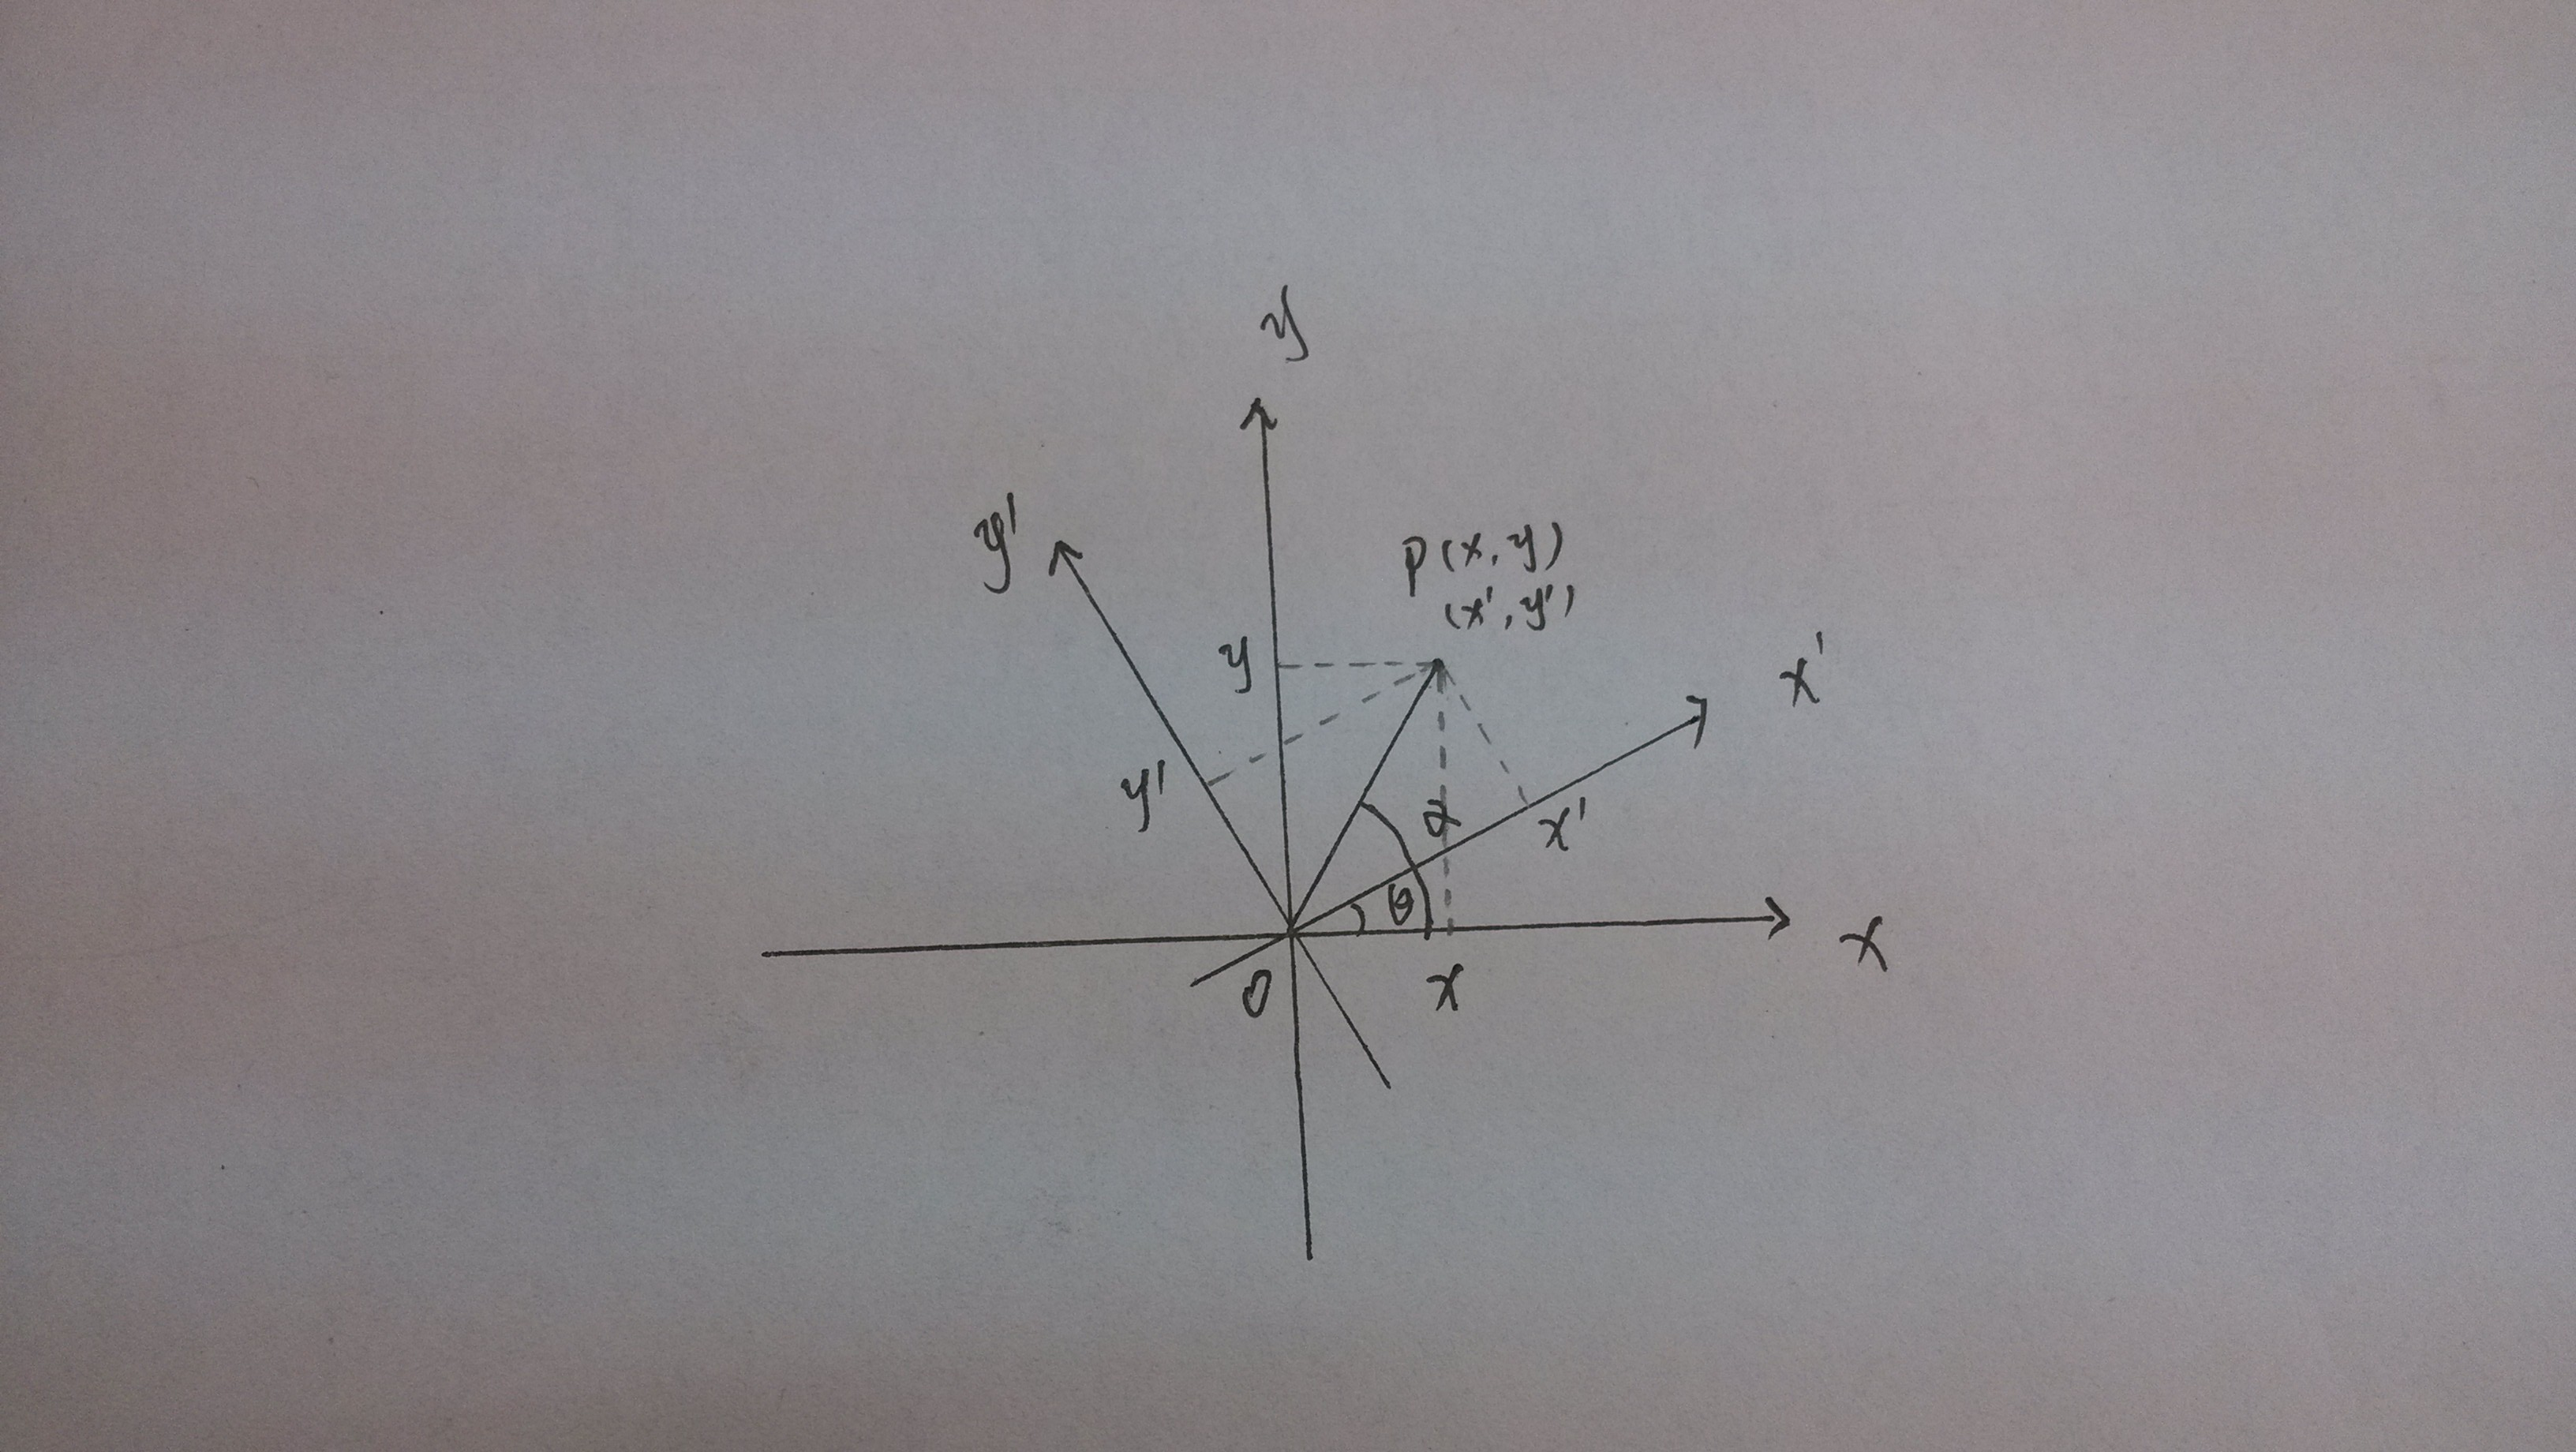
\includegraphics[width=3in,bb=885 550 2505 1470,clip]{f1}
\end{figure}
\end{frame}
\begin{frame}
因此有
$$\left[\begin{matrix}x'\\y'\end{matrix}\right]=\left[\begin{matrix}\cos\theta&\sin\theta\\-\sin\theta&\cos\theta\end{matrix}\right]\left[\begin{matrix}x\\y\end{matrix}\right],$$
或写成
$$\left[\begin{matrix}x\\y\end{matrix}\right]=\left[\begin{matrix}\cos\theta&-\sin\theta\\\sin\theta&\cos\theta\end{matrix}\right]\left[\begin{matrix}x'\\y'\end{matrix}\right].$$
\pause\vskip 10pt
\ \ \ \ 可以证明,任意一个行列式等于1的2阶正交矩阵总可以写成 \\$\left[\begin{matrix}\cos\theta&\sin\theta\\-\sin\theta&\cos\theta\end{matrix}\right]$的形式。
\end{frame}
\begin{frame}
\ \ \ \ 在平面直角坐标系下,一般二次曲线的方程可写成
$$a_{11}x^2+2a_{12}xy+a_{22}y^2+2a_1x+2a_2y+a_0=0,$$
其中二次项系数是不全为0的实数。
\vskip 5pt
\ \ \ \ 考虑实二次型$f(x,y)=a_{11}x^2+2a_{12}xy+a_{22}y^2$, 首先利用正交替换(即转轴变换)$\left[\begin{matrix}x'\\y'\end{matrix}\right]=\bm T\left[\begin{matrix}x\\y\end{matrix}\right]$可以把实二次型$f(x,y)$化成标准形,
\pause 即
$f(x,y)=\lambda_1x'^2+\lambda_2y'^2.$
这时,原二次曲线方程变成
$$\lambda_1x'^2+\lambda_2y'^2+2b_1x'+2b_2y'+b_0=0.$$
\ \ \ \ 最后,用配方法对方程作进一步化简,并作坐标平移就可以把二次曲线方程标准化了。
\pause\vskip 5pt
\ \ \ \ 因此,把二次曲线方程标准化的步骤如下:
\vskip 5pt
\ \ \ \ (1) 作坐标轴旋转消去$xy$项;
\vskip 5pt
\ \ \ \ (2) 作坐标平移。
\end{frame}
\begin{frame}
\ \ \ \ 二次曲线方程标准化有下面三种情形:
\vskip 5pt
\ \ \ \ (1) 若实二次型$f(x,y)$的秩为1,那么经过正交替换后$f(x,y)=\lambda x'^2$,其中$\lambda$为$f(x,y)$的唯一的非零特征值(另一个为0)。于是除了退化的情形外,原二次曲线代表一个抛物线。
\pause\vskip 5pt
\ \ \ \ (2) 若实二次型$f(x,y)$的秩为2且为不定的,那么经过正交替换后$f(x,y)=\lambda_1x'^2+\lambda_2y'^2$,其中$\lambda_1,\lambda_2$为$f(x,y)$的两个特征值,且$\lambda_1\lambda_2<0$. 于是除了退化的情形外,原二次曲线代表一个双曲线。
\pause\vskip 5pt
\ \ \ \ (3) 若实二次型$f(x,y)$的秩为2且为正定的(负定的),那么经过正交替换后$f(x,y)=\lambda_1x'^2+\lambda_2y'^2$,其中$\lambda_1,\lambda_2$为$f(x,y)$的两个特征值,且$\lambda_1\lambda_2>0$. 于是除了退化的情形外,原二次曲线代表一个椭圆。
\end{frame}
\begin{frame}\small
\ \ \ \ {\hei 例~1} 求平面上二次曲线方程
$$5x^2+4xy+2y^2-24x-12y+18=0$$
的标准方程,并作出其图形。
\pause\vskip 2pt
\ \ \ \ {\hei 解} 令$f(x,y)=5x^2+4xy+2y^2$,其对应的矩阵为$\bm A=\left[\begin{matrix}5&2\\2&2\end{matrix}\right]$,特征多项式为
$$|\lambda\bm E-\bm A|=\left|\begin{matrix}\lambda-5&-2\\-2&\lambda-2\end{matrix}\right|=\lambda^2-7\lambda+6=(\lambda-6)(\lambda-1),$$
故$\bm A$的特征值为6, 1.
\vskip 2pt
\ \ \ \ 把$\lambda=6$代入$(\lambda\bm E-\bm A)\bm X=\bm 0$,求出属于特征值$\lambda=6$的一个线性无关的特征向量$\left[\begin{matrix}2\\1\end{matrix}\right]$,再单位化得$\left[\begin{matrix}\frac{2}{\sqrt5}\\\frac{1}{\sqrt5}\end{matrix}\right]$.
\vskip 2pt
\ \ \ \ 把$\lambda=1$代入$(\lambda\bm E-\bm A)\bm X=\bm 0$,求出属于特征值$\lambda=1$的一个线性无关的特征向量$\left[\begin{matrix}-1\\2\end{matrix}\right]$,再单位化得$\left[\begin{matrix}-\frac{1}{\sqrt5}\\\frac{2}{\sqrt5}\end{matrix}\right]$.
\end{frame}
\begin{frame}\small
令$\bm T=\left[\begin{matrix}\frac{2}{\sqrt5}&-\frac{1}{\sqrt5}\\\frac{1}{\sqrt5}&\frac{2}{\sqrt5}\end{matrix}\right]$,则$\bm T$为正交矩阵,且在正交替换$\left[\begin{matrix}x\\y\end{matrix}\right]=\bm T\left[\begin{matrix}x'\\y'\end{matrix}\right]$下得到$f(x,y)=6x'^2+y'^2$,从而原二次曲线的方程化为
$$6x'^2+y'^2-12\sqrt5 x'+18=0,$$
配方,得
$$6(x'-\sqrt5)^2+y'^2=12,~~~~\mbox{即}~\frac{(x'-\sqrt5)^2}2+\frac{y'^2}{12}=1,$$
令$x''=x'-\sqrt5,~y''=y'$,则原二次曲线方程化成了标准方程
$$\frac{x''^2}2+\frac{y''^2}{12}=1.$$
\pause\ \ \ \ 原二次方程的图形是一个椭圆,其长轴在$y''$轴上,长、短半轴长分别为$2\sqrt3$和$\sqrt2$. 此时所作的坐标旋轴和平移总的坐标变换公式为
$$\left[\begin{matrix}x\\y\end{matrix}\right]=\bm T\left[\begin{matrix}x''+\sqrt5\\y''\end{matrix}\right].$$
\end{frame}
\begin{frame}{二次曲面方程的标准化}\small
\ \ \ \ 在空间直角坐标系下,一般二次曲面的方程可写成
$$a_{11}x^2+2a_{12}xy+2a_{13}xz+a_{22}y^2+2a_{23}yz+a_{33}z^2+2a_1x+2a_2y+2a_3z+a_4=0,$$
其中二次项系数是不全为0的实数。
\vskip 5pt
\ \ \ \ 令$f(x,y,z)=a_{11}x^2+2a_{12}xy+2a_{13}xz+a_{22}y^2+2a_{23}yz+a_{33}z^2$,其对应的矩阵$\bm A=(a_{ij})_{3\times3}$为实对称矩阵。由定理5.7,存在正交矩阵$\bm T$,使
$$\bm T'\bm{AT}=\bm T^{-1}\bm{AT}=\left[\begin{matrix}\lambda_1&&\\&\lambda_2&\\&&\lambda_3\end{matrix}\right].$$
其中$\lambda_1,\lambda_2,\lambda_3$为$\bm A$的特征值。
\vskip 5pt
\ \ \ \ 作转轴变换$\bm X=\bm{TY}$,其中$\bm Y=(x',y',z')'$,从而得到$f(x,y,z)=\lambda_1x'^2+\lambda_2y'^2+\lambda_3z'^2$.
\end{frame}
\begin{frame}
\ \ \ \ 原二次曲面方程化为
$$\lambda_1x'^2+\lambda_2y'^2+\lambda_3z'^2+2b_1x'+2b_2y'+2b_3z'+b_4=0.$$
\ \ \ \ 二次曲面方程标准化有下面三种情形:
\vskip 5pt
\ \ \ \ (1) 若实二次型$f(x,y)$的秩为1。不妨设$\lambda_1\neq0,~\lambda_2=\lambda_3=0$,不讨论退化的情形,假设$b_2,b_3$不全为0. 先作转轴变换
$$\left[\begin{matrix}x'\\y'\\z'\end{matrix}\right]=\left[\begin{matrix}1&0&0\\0&\frac{b_2}{\sqrt{b_2^2+b_3^2}}&\frac{b_3}{\sqrt{b_2^2+b_3^2}}
\\0&-\frac{b_3}{\sqrt{b_2^2+b_3^2}}&\frac{b_2}{\sqrt{b_2^2+b_3^2}}\end{matrix}\right]^{-1}\left[\begin{matrix}x''\\y''\\z''\end{matrix}\right],$$
则二次曲面方程化为~$\lambda_1x''^2+2b_1x''+2\sqrt{b_2^2+b_3^2}y''+b_4=0$,再配方作平移变换就化成标准方程~$u^2=2pv,~p\neq0$为常数。它代表一个抛物柱面。
\end{frame}
\begin{frame}
\ \ \ \ (2) 若实二次型$f(x,y)$的秩为2,不妨设$\lambda_1\neq0,~\lambda_2\neq0,~\lambda_3=0$. 若$b_3=0$, 经过配方作平移变换后二次曲面方程可化为$\lambda_1x''^2+\lambda_2y''^2=c_0$. 不讨论退化的情形,假设$c_0\neq0$,当$\lambda_1,\lambda_2$同号时,它代表一个椭圆柱面;当异号时,它代表一个双曲柱面。
\pause\vskip 5pt
\ \ \ \ 若$b_3\neq0$, 经过配方作平移变换后二次曲面方程可化为$\lambda_1x''^2+\lambda_2y''^2=c_0z,~c_0\neq0$. 当$\lambda_1,\lambda_2$同号时,它代表一个椭圆抛物面;当异号时,它代表一个双曲抛物面。
\pause\vskip 5pt
\ \ \ \ (3) 若实二次型$f(x,y)$的秩为3,即$\lambda_1,\lambda_2,\lambda_3$均非零。配方消去一次项,再平移后二次曲面方程化为$\lambda_1x''^2+\lambda_2y''^2+\lambda_3z''^2=c_0$. 不讨论退化的情形,假设$c_0\neq0$,当$\lambda_1,\lambda_2,\lambda_3$同号时,它代表一个椭球面;当$\lambda_1,\lambda_2,\lambda_3$符号不完全相同时,它代表一个单叶或双叶双曲面。
\end{frame}

\section{复习要点}
\begin{frame}{第一章}
\begin{itemize}
  \item 0.1 复数、数域
  \item 1.4 向量数量积、向量积、混合积的定义及性质
  \item 1.5 向量数量积、向量积、混合积、长度、夹角的坐标表示\\
  \ \ \ \ \ 向量平行(共线)、垂直、共面的坐标关系
  \item 1.6 平面方程的四种形式:点法式、一般式、三点式、截距式\\
  \ \ \ \ \ 点到平面的距离公式和面与面之间的关系
  \item 1.7 直线方程的四种形式:参数式、点向式、一般式、两点式\\
  \ \ \ \ \ 直线之间的关系、直线和平面之间的关系\\
  \ \ \ \ \ 点到直线的距离公式、异面直线的距离公式
\end{itemize}
\end{frame}

\begin{frame}{第二章}
\begin{itemize}
  \item 2.1 行列式、余子式、代数余子式的定义
  \item 2.2 行列式的展开定理及6个性质,\\
  \ \ \ \ \ 行列式的转置,上、下三角形行列式\\
  \ \ \ \ \ 行列式的计算
  \item 3.3 拉普拉斯定理、克拉默法则及推论
\end{itemize}
\end{frame}

\begin{frame}{第三章}
\begin{itemize}
  \item 3.1 几类特殊的矩阵
  \item 3.2 矩阵的乘法及性质、矩阵转置和乘法的结合\\
  \ \ \ \ \ 对称矩阵和反对称矩阵、方阵的幂\\
  \ \ \ \ \ 分块矩阵的乘法,准对角矩阵的乘法
  \item 3.3 逆矩阵的定义、方阵的行列式及性质\\
  \ \ \ \ \ 伴随矩阵的定义及性质、非退化矩阵的定义\\
  \ \ \ \ \ 矩阵可逆的充要条件及判定、可逆矩阵的性质\\
  \ \ \ \ \ 利用伴随矩阵求逆矩阵\\
  \item 3.4 初等变换和初等矩阵之间的关系\\
  \ \ \ \ \ 矩阵的标准形及相关结论、矩阵的等价\\
  \ \ \ \ \ 矩阵可逆的充要条件、矩阵等价的充要条件\\
  \ \ \ \ \ 利用行初等变换求逆矩阵
\end{itemize}
\end{frame}

\begin{frame}{第四章}\small
\begin{itemize}
  \item 4.1 增广矩阵的定义、消元法\\
  \ \ \ \ \ 线性方程组解的三种情况\\
  \ \ \ \ \ 齐次线性方程组有非零解的条件
  \item 4.2 向量空间、欧氏空间、子空间、齐次方程组解空间的定义\\
  \ \ \ \ \ 内积、长度、夹角、向量正交(垂直)的定义\\
  \ \ \ \ \ 柯西不等式
  \item 4.3 线性表出、线性相关(无关)、向量组等价、基本向量组的定义\\
  \ \ \ \ \ 线性相关和线性无关的判定(充要条件)\\
  \ \ \ \ \ 例9、例10、定理4.5\\
  \ \ \ \ \ 线性表出和线性相关之间的联系及推论
  \item 4.5 极大线性无关组的定义及判定、性质,向量组的秩\\
   \ \ \ \ \ 矩阵的秩及其性质\\
    \ \ \ \ \ 求极大线性无关组和矩阵的秩\\
   \ \ \ \ \ 可逆矩阵的秩、满秩矩阵的定义\\
   \ \ \ \ \ 利用k阶子式求矩阵的秩\\
    \ \ \ \ \ 可逆矩阵的一些等价描述
\end{itemize}
\end{frame}

\begin{frame}{第四章}
\begin{itemize}
 \item 4.6 线性方程组有解判定定理:引理、定理4.15、定理4.16
 \item 4.7 齐次线性方程组有基础解系的充要条件:定理4.17、推论1、2\\
 \ \ \ \ \ 齐次线性方程组解空间的维数\\
 \ \ \ \ \ 利用系数矩阵求解齐次线性方程组的一般解及基础解系\\
 \ \ \ \ \ 非齐次线性方程组和导出组的解之间的关系\\
 \ \ \ \ \ 利用增广矩阵求解非齐次线性方程组的一般解:特解,导出组的基础解系
\end{itemize}
\end{frame}

\begin{frame}{第五章}
\begin{itemize}
  \item 5.1 特征值和特征向量、特征子空间的定义\\
  \ \ \ \ \ 特征值和矩阵的关系\\
  \ \ \ \ \ 求解矩阵的特征值和特征向量
  \item 5.2 矩阵相似的定义和性质\\
  \ \ \ \ \ 矩阵可以对角化的充要条件及证明\\
  \ \ \ \ \ 几何重数和代数重数的定义\\
  \ \ \ \ \ 定理5.4、定理5.5、推论1、2\\
  \ \ \ \ \ 求可逆矩阵$\bm C$使$\bm A$对角化
  \item 5.3 正交向量组的相关定义及性质\\
  \ \ \ \ \ 正交矩阵的定义及性质,正交矩阵和标准正交基的关系\\
  \ \ \ \ \ 施密特正交化方法\\
   \ \ \ \ \ 酉空间的内积及其性质,内积与矩阵之间的关系\\
   \ \ \ \ \ 引理1、2,定理5.8\\
   \ \ \ \ \ 求正交矩阵$\bm T$使实对称矩阵$\bm A$对角化
\end{itemize}
\end{frame}


%=====================================================frame8=========================================


\begin{frame}
\begin{center}
{\textcolor[rgb]{0.50,0.00,1.00}{\textbf{\xiaoerhao{Thanks for your attention!}}}}\bigskip
\end{center}
\end{frame}
\end{CJK}
\end{document}


